\documentclass[9pt]{article}

\usepackage{amsmath}
\usepackage{tcolorbox}
% `parskip` removes indentation for all paragraphs: http://tex.stackexchange.com/a/55016
\usepackage{parskip}
% Allows us to color rows / cols of a table.
% See https://texblog.org/2011/04/19/highlight-table-rowscolumns-with-color/
\usepackage{color, colortbl}
\graphicspath{{images/ps4/}}

\usepackage{hyperref}

\leftmargin=0.25in
\oddsidemargin=0.25in
\textwidth=6.0in
\topmargin=-0.25in
\textheight=9.25in

\definecolor{Gray}{gray}{0.9}

\begin{document}

\begin{center}
  \large\textbf{MIT 18.01 Problem Set 4 Unofficial Solutions}
\end{center}

\begin{tcolorbox}
  \textbf{Q1a)} Use the mean value property to show that if $f(0) = 0$ and $f'(x) \geq 0$, then $f(x) \geq 0$ for all $x \geq 0$.
\end{tcolorbox}

For any $x > 0$, $f(x) = f(0) + f'(c)(x - 0)$, for some $0 < c < x$

Since $f'(x) \geq 0$ for all $x$, then for all $x > 0$, $f(x) \geq f(0)$.

Since $f(x) \geq f(0) \geq 0$ for all $x > 0$, then $f(x) \geq 0$ for all $x > 0$.

Since $f(0) = 0$ and $f(x) \geq 0$ for all $x > 0$, then $f(x) \geq 0$ for all $x \geq 0$.


\begin{tcolorbox}
  \textbf{Q1b)} Deduce from part (a) that $ln(1 + x) \leq x$ for $x \geq 0$. Hint: Use $f(x) = x - ln(1 + x)$.
\end{tcolorbox}

Let $f(x) = x - ln(1 + x)$

Then $f(0) = 0 - ln(1 + 0) = 0 - 0 = 0$

$f'(x) = 1 - \frac{1}{1 + x}$

For all $x \geq 0$, $1 + x \geq 1$ and $\frac{1}{1 + x} \leq 1$ and $1 - \frac{1}{1 + x} \geq 0$

Since $f'(x) = 1 - \frac{1}{1 + x} \geq 0$, therefore $f'(x) \geq 0$ for $x \geq 0$.

By 1(a), $f(x) = x - ln(1 + x) \geq 0$ for $x \geq 0$

Then $x \geq ln(1 + x)$ for $x \geq 0$


\begin{tcolorbox}
  \textbf{Q1c)} Use the same method as in (b) to show $ln(1 + x) \geq x - x^2 / 2$ and $ln(1 + x) \leq x - x^2 / 2 + x^3 / 3$ for $x \geq 0$.
\end{tcolorbox}

Let $f_1(x) = ln(1 + x) - x + \frac{x^2}{2}$

$f_1(0) = ln(1 + 0) - 0 + \frac{0^2}{2} = 0$

$f_1'(x) = \frac{1}{1 + x} - 1 + x = \frac{1 - (1 + x) + x(1 + x)}{1 + x} = \frac{1 - 1 - x + x + x^2}{1 + x} = \frac{x^2}{1 + x}$

Since $1 + x \geq 1$ for all $x \geq 0$ and $x^2 \geq 0$ for all $x \geq 0$, then $f_1'(x) = \frac{x^2}{1 + x} \geq 0$ for all $x \geq 0$.

By 1(a), $f_1(x) \geq 0$ for all $x \geq 0$, which is equivalent to $ln(1 + x) - x - \frac{x^2}{2} \geq 0$ for all $x \geq 0$. Hence $ln(1 + x) \geq x - \frac{x^2}{2}$ for all $x \geq 0$.
\\

Let $f_2(x) = x - \frac{x^2}{2} + \frac{x^3}{3} - ln(1 + x)$

$f_2(0) = 0 - \frac{0^2}{2} + \frac{0^3}{3} - ln(1 + 0) = 0$

$f_2'(x) = 1 - x + x^2 - \frac{1}{1 + x} = \frac{1(1 + x) - x(1 + x) + x^2 (1 + x) - 1}{1 + x} = \frac{1 + x - x - x^2 + x^2 + x^3}{1 + x} = \frac{x^3}{1 + x}$

Since $1 + x \geq 1$ for all $x \geq 0$ and $x^3 \geq 0$ for all $x \geq 0$, then $f_2'(x) = \frac{x^3}{1 + x} \geq 0$ for all $x \geq 0$.

By 1(a), $f_2(x) = x - \frac{x^2}{2} + \frac{x^3}{3} - ln(1 + x) \geq 0$ for all $x \geq 0$. Hence $x - \frac{x^2}{2} + \frac{x^3}{3} \geq ln(1 + x)$ for all $x \geq 0$.


\begin{tcolorbox}
  \textbf{Q1d)} Find the pattern in (b) and (c) and make a general conjecture.
\end{tcolorbox}

General conjecture:

$ln(1 + x) \leq x - \frac{x^2}{2} + \frac{x^3}{3} + ... + \frac{x^{2n + 1}}{2n + 1} = \sum\limits_{k=1}^{2n + 1} (-1)^{k+1} \frac{x^k}{k}$ for all $x \geq 0, n \geq 0$

$ln(1 + x) \geq x - \frac{x^2}{2} + \frac{x^3}{3} + ... + \frac{x^{2n}}{2n} = \sum\limits_{k=1}^{2n} (-1)^{k+1} \frac{x^k}{k}$ for all $x \geq 0, n \geq 1$

Let $f_1(x) = (\sum\limits_{k=1}^{2n + 1} (-1)^{k+1} \frac{x^k}{k}) - ln(x + 1)$ for any $n \geq 1$.

$f_1(0) = (\sum\limits_{k=1}^{2n + 1} (-1)^{k+1} \frac{0^k}{k}) - ln(0 + 1) = 0$

\begin{align*}
  f_1'(x) &= (\sum\limits_{k=1}^{2n + 1} (-1)^{k+1} x^{k-1}) - \frac{1}{x + 1} \\
          &= \frac{(x+1)(\sum\limits_{k=1}^{2n + 1} (-1)^{k+1} x^{k-1}) - 1}{x + 1} \\
          &= \frac{(\sum\limits_{k=1}^{2n + 1} (-1)^{k+1} (x^k + x^{k - 1})) - 1}{x + 1} \\
          &= \frac{(x^1 + x^0) - (x^2 + x^1) + ... + (-1)^{2n + 1 + 1}(x^{2n + 1} + x^{2n}) - 1}{x + 1} \\
          &= \frac{x^0 + x^{2n + 1} - 1}{x + 1} \\
          &= \frac{x^{2n + 1}}{x + 1}
\end{align*}

Since $x + 1 \geq 1$ for $x \geq 0$ and $x^{2n + 1} \geq 0$ for $n \geq 0, x \geq 0$, then $f_1'(x) = \frac{x^{2n + 1}}{x + 1} \geq 0$ for all $x \geq 0$.

By 1(a), $f_1(x) = (\sum\limits_{k=1}^{2n+1} (-1)^{k+1} \frac{x^k}{k}) - ln(x + 1) \geq 0$ for all $x \geq 0, n \geq 0$. Hence $ln(x + 1) \leq \sum\limits_{k=1}^{2n+1} (-1)^{k+1} \frac{x^k}{k}$ for all $x \geq 0, n \geq 0$.
\\
\\

Let $f_2(x) = ln(x + 1) - \sum\limits_{k=1}^{2n} (-1)^{k+1} \frac{x^k}{k}$ for any $n \geq 0$.

$f_2(0) = ln(0 + 1) - \sum\limits_{k=1}^{2n} (-1)^{k+1} \frac{0^k}{k} = 0$

\begin{align*}
  f_2'(x) &= \frac{1}{x + 1} - \sum\limits_{k=1}^{2n} (-1)^{k+1} x^{k-1} \\
          &= \frac{1 - (x + 1)\sum\limits_{k=1}^{2n} x^{k - 1}}{x + 1} \\
          &= \frac{1 - \sum\limits_{k=1}^{2n}(x^k + x^{k - 1})}{x + 1} \\
          &= \frac{1 - ((x^1 + x^0) - (x^2 + x^1) + ... + (-1)^{2n + 1}(x^{2n} + x^{2n - 1}))}{x + 1} \\
          &= \frac{1 - (x^0 - x^{2n})}{x + 1} \\
          &= \frac{x^{2n}}{x + 1}
\end{align*}

For $x \geq 0$, $x + 1 \geq 1$ and $x^{2n} \geq 0$ for $x \geq 0, n \geq 1$. Hence $f_2'(x) = \frac{x^{2n}}{x + 1} \geq 0$ for $n \geq 1, x \geq 0$.

By 1(a), $f_2(x) = ln(x + 1) - \sum\limits_{k=1}^{2n} (-1)^{k+1} x^{k-1} \geq 0$ for all $n \geq 1, x \geq 0$.

Then $ln(x + 1) \geq \sum\limits_{k=1}^{2n} (-1)^{k+1} x^{k-1}$ for all $n \geq 1, x \geq 0$.


\begin{tcolorbox}
  \textbf{Q1e)} Show that $ln(1 + x) \leq x$ for $-1 < x \leq 0$. (Use the change of variable $u = -x$.)
\end{tcolorbox}

Let $u = -x$. Then $x = -u$.

We want to show that $ln(1 - u) \leq -u$ for $0 \leq u < 1$.

Let $f(u) = -u - ln(1 - u)$

$f(0) = -0 - ln(1 - 0) = 0$

$f'(u) = -1 - \frac{-1}{1 - u} = -1 + \frac{1}{1-u} = \frac{-1(1-u) + 1}{1 - u} = \frac{u - 1 + 1}{1 - u} = \frac{u}{1 - u}$

Since $0 \leq u < 1$, then $1 - u > 0$. Hence $f'(u) = \frac{u}{1 - u} \geq 0$ for $0 \leq u < 1$

By 1(a), $f(u) = -u - ln(1 - u) \geq 0$ for $0 \leq u < 1$.

Then $f(x) = -(-x) - ln(1 - (-x)) = x - ln(1 + x) \geq 0$ for $0 \leq -x < 1$ or $-1 < x \leq 0$.

Hence $ln(1 + x) \leq x$ for $-1 < x \leq 0$


\begin{tcolorbox}
  \textbf{Q2a)} Do 5.3/68
\end{tcolorbox}

I do not have the textbook. Skipped.


\begin{tcolorbox}
  \textbf{Q2b)} Show that both of the following integrals are correct, and explain.

  \begin{align*}
    \int tan x\ sec^2 x\ dx = (1/2) tan^2 x; \int tan x\ sec^2 x\ dx = (1/2) sec^2 x
  \end{align*}
\end{tcolorbox}

Let $u = tan\ x$. We have

\begin{align*}
  \int tan x\ sec^2 dx &= \int (sec^2 x)\ tan x\ dx \\
                       &= \int u'\ u\ du \\
                       &= \frac{1}{2} u^2 + c \\
                       &= \frac{1}{2} tan^2 x + c
\end{align*}

Now we want to prove that $\int tan x\ sec^2 x\ dx = (1/2) sec^2 x$. Let $u = sec\ x$. Then $\int u' \ u\ du = \frac{1}{2}u^2 + c = \frac{1}{2} sec^2 x + c$


\begin{tcolorbox}
  \textbf{Q3)} (Lec 16, 6 pts: 3 + 3)\\
  a) Do 8.6/5 (answer in back of book)\\
  b) Do 8.6/6 (optional?)
\end{tcolorbox}

I do not have the textbook. Skipped.


\begin{tcolorbox}
  \textbf{Q4)} (Lec 16, 7 pts: 2 + 3 + 2) Do 3F-5abc\\
  \\
  3F-5 Air pressure satisfies the differential equation $dp/dh = -(.13)p$, where $h$ is the altitude from sea level measured in kilometres.\\
  a) At sea level the pressure is $1kg/cm^2$. Solve the equation and find the pressure at the top of Mt. Everest (10 km).
\end{tcolorbox}

\begin{align*}
  \frac{dp}{dh} &= -(.13)p\\
  \frac{1}{p} dp &= -.13 dh\\
  \int \frac{1}{p} dp &= \int -.13 dh\\
  ln\ p &= -.13h + c\\
  p &= e^{-.13h + c}\\
  p &= e^{-.13h} \cdot e^c\\
  p &= A e^{-.13h}
\end{align*}

where $A = e^c$. When $h = 0, p = 1$ (sea level pressure is $1$). Then $p = 1 = A e^{-.13(0)} = A$. Hence $p = A e^{-.13h} = 1 \cdot e^{-.13h} = e^{-.13h}$

At the top of Mt Everest, $p = e^{-.13(10)} \approx 0.2725\ kg/cm^2$

\begin{tcolorbox}
  \textbf{Q4)} (Lec 16, 7 pts: 2 + 3 + 2) Do 3F-5abc\\
  \\
  3F-5 b) Find the difference in pressure between the top and bottom of the Green building. (Pretend it's 100 meters tall starting at sea level.) Compute the numerical value using a calculator. Then use instead the linear approximation to $e^x$ near $x = 0$ to estimate the percentage drop in pressure from the bottom to the top of the Green Building.
\end{tcolorbox}

Difference = $e^{-.13(0.1)} - e^{-13(0)} = e^{-.013} - 1 \approx -0.012915865\ kg/cm^2$

Linear approximation to $e^x$ near $x = 0$ is $1 + x$. But because we are dealing with $e^{-.13h}$, for $h \approx 0$, $e^{-.13h} \approx e^{-.13(0)} + -.13e^{-.13(0)}h = 1 - .13h$

Pressure at top - Pressure at bottom $\approx 1 - .13(0.1) - 1 \approx -0.013\ kg/cm^2$
\begin{tcolorbox}
  \textbf{Q4)} (Lec 16, 7 pts: 2 + 3 + 2) Do 3F-5abc\\
  \\
  3F-5 c) Use the linear approximation $\Delta p \approx p'(0) \Delta h$ and compute $p'(0)$ directly from the differential equation to find the drop in pressure from the bottom to top of the Green Building. Notice that this gives an answer without even knowing the solution to the differential equation. Compare with the approximation in part (b). What does the linear approximation $p'(0)\Delta h$ give for the pressure at the top of Mt. Everest?
\end{tcolorbox}

\begin{align*}
  \Delta p &\approx p'(0)\Delta h\\
  \frac{\Delta p}{\Delta h} &\approx p'(0)\\
  \lim_{\Delta h \rightarrow 0} \frac{dp}{dh} &= \frac{dp}{dh}\\
  \frac{\Delta p}{\Delta h} &\approx \frac{dp}{dh} = -.13p
\end{align*}

We will use $p'(0) \approx \frac{\Delta p}{\Delta h} \approx -.13p$. When $h = 0, p = 1$. Hence $1 = p'(0) \approx -.13p = -.13(1) = -.13$, which implies that every kilometre increase in altitude causes pressure to decrease by $-.13\ kg/cm^2$.

Drop in pressure from bottom to top of green building = $-(-.13(0.1)) = 0.013\ kg/cm^2$ which was exactly the same as what we got using the linear approximation in part (b).

For pressure at top of Mt Everest, we have $\Delta h = 10$. Hence

\begin{align*}
  p(0) + p'(0)\Delta h &= 1 + -.13(10)\\
                       &= 1 - 1.3\\
                       &= -0.3\ kg/cm^2
\end{align*}

which is totally incorrect because $\Delta h = 10$ is much bigger than $0$ and causes the approximation to be wildly inaccurate.


\begin{tcolorbox}
  \textbf{Q5)} Calculate $\int_{0}^{1} e^x dx$ using lower Riemann sums. (You will need to sum a geometric series to get a usable formula for the Riemann sum. To take the limit of Riemann sums, you will need to evaluate $\lim\limits_{n \to \infty} n(e^{1/n} - 1)$, which can be done using the standard linear approximation to the exponential function.)
\end{tcolorbox}

\begin{align*}
  \int_{0}^{1} e^x dx &= \lim\limits_{n \to \infty} \sum_{k=0}^{n-1} e^{\frac{k}{n}} \frac{1}{n}\\
                      &= \lim\limits_{n \to \infty} \frac{1}{n} \sum_{k=0}^{n-1} e^{\frac{k}{n}}\\
                      &= \lim\limits_{n \to \infty} \frac{1}{n} \sum_{k=0}^{n-1} (e^{\frac{1}{n}})^k\\
                      &= \lim\limits_{n \to \infty} \frac{1}{n} \cdot \frac{1 - (e^{\frac{1}{n}})^n}{1 - e^{\frac{1}{n}}}\\
                      &= \lim\limits_{n \to \infty} \frac{1}{n} \cdot \frac{1 - e}{1 - e^\frac{1}{n}}\\
                      &= \lim\limits_{n \to \infty} \frac{1 - e}{n(1 - e^{\frac{1}{n}})}
\end{align*}

The linear approximation to $e^x$ near $x = 0$ is $e^0 + e^0 x = 1 + x$. Since $n \rightarrow \infty, \frac{1}{n} \rightarrow 0$ and $e^{\frac{1}{n}} \approx 1 + \frac{1}{n}$. Then

\begin{align*}
  \int_{0}^{1} e^x dx &= \lim\limits_{n \to \infty} \frac{1 - e}{n(1 - e^{\frac{1}{n}})}\\
                      &\approx \lim\limits_{n \to \infty} \frac{1 - e}{n(1 - (1 + \frac{1}{n}))}\\
                      &= \lim\limits_{n \to \infty} \frac{1 - e}{n(-\frac{1}{n})}\\
                      &= \lim\limits_{n \to \infty} \frac{1 - e}{-1}\\
                      &= \lim\limits_{n \to \infty} e - 1\\
                      &= e - 1
\end{align*}


\begin{tcolorbox}
  \textbf{Q6) More about the hypocycloid} We use differential equations to find the curve with the property that the potrion of its tangent line in the first quadrant has fixed length.\\
  \\
  a) Suppose that a line through the point $(x_0, y_0)$ has slope $m_0$ and that the point is in the first quadrant. Let $L$ denote the length of the portion of the line in the first quadrant. Calculate $L^2$ in terms of $x_0, y_0$ and $m_0$. (Do not expand or simplify.)
\end{tcolorbox}

Equation of tangent line is given by $y - y_0 = m_0(x - x_0)$. When $x = 0$

\begin{align*}
  y - y_0 &= m_0(0 - x_0)\\
  y &= -m_0 x_0 + y_0
\end{align*}

When $y = 0$,

\begin{align*}
  0 - y_0 &= m_0(x - x_0)\\
  -\frac{y_0}{m_0} &= x - x_0\\
  x &= x_0 - \frac{y_0}{m_0}
\end{align*}

Substituting the above equations for $x$ and $y$ into $L^2 = x^2 + y^2$, we have

\begin{align*}
  L^2 &= x^2 + y^2\\
      &= (x_0 - \frac{y_0}{m_0})^2 + (-m_0 x_0 + y_0)^2
\end{align*}


\begin{tcolorbox}
  \textbf{Q6b)} Suppose that $y = f(x)$ is a graph on $0 \leq x \leq L$ satisfying $f(0) = L$ and $f(L) = 0$ and such that the portion of each tangent line to the graph in the first quadrant has the same length $L$. Find the differential equation that $f$ satisfies. Express it in terms of $L, x, y$ and $y' = dy/dx$. (Hints: This requires only thought, not computation. Note that $y = f(x), y' = f'(x)$. Don't take square roots, the expression using $L^2$ is much easier to use. Don't expand or simplify; that would make things harder in the next step.)
\end{tcolorbox}

\begin{center}
  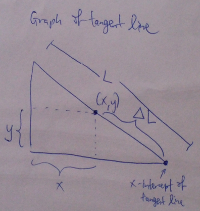
\includegraphics[]{q6b.jpg}
\end{center}

Apologies for the poor quality image.

Let the x-intercept of the tangent line be point $d$. Given a point $(x, y)$ on the tangent line, we have

\begin{align*}
  \frac{dy}{dx} &= \frac{0 - y}{d - x}\\
  d - x &= \frac{-y}{\frac{dy}{dx}}\\
  d &= x - \frac{y}{\frac{dy}{dx}}
\end{align*}

We also see from the diagram that $(\Delta L)^2 = y^2 + (d - x)^2 = y^2 + (x - \frac{y}{\frac{dy}{dx}} - x)^2 = y^2 + (-\frac{y}{\frac{dy}{dx}})^2 = y^2 + (\frac{y}{\frac{dy}{dx}})^2$

The y-intercept of the graph is $y - x \cdot \frac{dy}{dx}$. This is also the height of the triangle in the diagram. Using similar triangles, we have

\begin{align*}
  \frac{y}{\Delta L} &= \frac{y - x \cdot \frac{dy}{dx}}{L}\\
  (\frac{y}{\Delta L})^2 &= (\frac{y - x \cdot \frac{dy}{dx}}{L})^2
\end{align*}

Substituting $(\Delta L)^2 = y^2 + (\frac{y}{\frac{dy}{dx}})^2$ which we got above:

\begin{align*}
  (\frac{y}{\Delta L})^2 &= (\frac{y - x \cdot \frac{dy}{dx}}{L})^2\\
  \frac{y^2}{y^2 + \frac{y^2}{(\frac{dy}{dx})^2}} &= (\frac{y - x \cdot \frac{dy}{dx}}{L})^2\\
  L^2 y^2 &= (y - x \cdot \frac{dy}{dx})^2 (y^2  + \frac{y^2}{(\frac{dy}{dx})^2})
\end{align*}


\begin{tcolorbox}
  \textbf{Q6c)} Differentiate the equation in part (b) with respect to $x$. Simplify and write in the form\\
  \begin{center}
    (something)$(xy' - y)y'' = 0$
  \end{center}

  \ \\
  (This starts out looking horrendous, but simplifies considerably.)
\end{tcolorbox}

\begin{align*}
  L^2 y^2 &= (y - x \cdot \frac{dy}{dx})^2 (y^2  + \frac{y^2}{(\frac{dy}{dx})^2})\\
  L^2 y^2 &= (y^2 - 2xy \cdot \frac{dy}{dx} + x^2 \cdot (\frac{dy}{dx})^2) (y^2 + \frac{y^2}{(\frac{dy}{dx})^2})\\
          &= y^4 + \frac{y^4}{(\frac{dy}{dx})^2} - 2xy^3 \cdot \frac{dy}{dx} - \frac{2xy^3}{\frac{dy}{dx}} + x^2y^2 \cdot (\frac{dy}{dx})^2 + x^2 y^2
\end{align*}

Differentiate implicitly with respect to $x$,

\begin{align*}
  L^2 \cdot 2y \cdot y' &= 4y^3 \cdot y' + \frac{4y^3(y')(y')^2 - y^4 \cdot 2y'(y'')}{(y')^4} - 2y^3y' - 6xy^2(y')^2 - 2xy^3y'' - \frac{2y^3y' + 6xy^2(y')^2 - 2xy^3y''}{(y')^2}\\
                        &\ \ \ + 2xy^2(y')^2 + 2x^2y(y')^3 + 2x^2y^2y'y'' + 2xy^2 + 2x^2yy'\\
                        &= 2y^3y' + \frac{4y^3(y')^3 - 2y^4y'y''}{(y')^4} - 4xy^2(y')^2 - 2xy^3y'' - \frac{2y^3y' + 6xy^2(y')^2 - 2xy^3y''}{(y')^2} + 2x^2y(y')^3\\
                        &\ \ \ + 2x^2y^2y'y'' + 2xy^2 + 2x^2yy'\\
                        &= \frac{1}{(y')^4}(2y^3(y')^5 + 4y^3(y')^3 - 2y^4y'y'' - 4xy^2(y')^6 - 2xy^3(y')^4y'' - 2y^3(y')^3 - 6xy^2(y')^4 + 2xy^3(y')^2y''\\
                        &\ \ \ + 2x^2y(y')^7 + 2x^2y^2(y')^5y'' + 2xy^2(y')^4 + 2x^2y(y')^5)
\end{align*}
\begin{align*}
  L^2 \cdot 2y \cdot y' \cdot (y')^4 &= 2y^3(y')^5 + 4y^3(y')^3 - 2y^4y'y'' - 4xy^2(y')^6 - 2xy^3(y')^4y'' - 2y^3(y')^3 - 6xy^2(y')^4 + 2xy^3(y')^2y''\\
                        &\ \ \ + 2x^2y(y')^7 + 2x^2y^2(y')^5y'' + 2xy^2(y')^4 + 2x^2y(y')^5
\end{align*}

In part (a), we got the result $L^2 = (x_0 - \frac{y_0}{m_0})^2 + (-m_0 x_0 + y_0)^2$ for any point $(x_0, y_0)$ on the tangent. Rewriting $m_0$ as $y'$, this becomes $L^2 = (x_0 - \frac{y_0}{y'})^2 + (-y' x_0 + y_0)^2$. Substituting the point $x_0 = x, y_0 = y$ for some point $(x, y)$ on the tangent line, this becomes $L^2 = (x - \frac{y}{y'})^2 + (-y' x + y)^2 = (y - xy')^2 + (x - \frac{y}{y'})^2$. Substituting that into $L^2 \cdot 2y \cdot y' \cdot (y')^4$, we have

\begin{align*}
  L^2 \cdot 2y \cdot y' \cdot (y')^4 &= ((y - xy')^2 + (x - \frac{y}{y'})^2) \cdot 2y \cdot y' \cdot (y')^4\\
                                     &= 2(y^2 - 2xyy' + x^2(y')^2 + x^2 - \frac{2xy}{y'} + \frac{y^2}{(y')^2}) \cdot y \cdot (y')^5\\
                                     &= 2y^3(y')^5 - 4xy^2(y')^6 + 2x^2y(y')^7 + 2x^2y(y')^5 - 4xy^2(y')^4 + 2y^3(y')^3
\end{align*}

Then
\begin{align*}
  L^2 \cdot 2y \cdot y' \cdot (y')^4 &= 2y^3(y')^5 + 4y^3(y')^3 - 2y^4y'y'' - 4xy^2(y')^6 - 2xy^3(y')^4y'' - 2y^3(y')^3 - 6xy^2(y')^4 + 2xy^3(y')^2y''\\
                        &\ \ \ + 2x^2y(y')^7 + 2x^2y^2(y')^5y'' + 2xy^2(y')^4 + 2x^2y(y')^5
\end{align*}

becomes
\begin{align*}
  &2y^3(y')^5 - 4xy^2(y')^6 + 2x^2y(y')^7 + 2x^2y(y')^5 - 4xy^2(y')^4 + 2y^3(y')^3 \\
  &= 2y^3(y')^5 + 4y^3(y')^3 - 2y^4y'y'' - 4xy^2(y')^6 - 2xy^3(y')^4y'' - 2y^3(y')^3 - 6xy^2(y')^4 + 2xy^3(y')^2y''\\
  &\ \ \ + 2x^2y(y')^7 + 2x^2y^2(y')^5y'' + 2xy^2(y')^4 + 2x^2y(y')^5
\end{align*}

which simplifies to

\begin{align*}
  0 = -2y^4y'y'' - 2xy^3(y')^4y'' + 2xy^3(y')^2y'' + 2x^2y^2(y')^5y''\\
  (y^3y' + xy^2(y')^4)(xy' - y)y'' = 0
\end{align*}


\begin{tcolorbox}
  \textbf{Q6d)} Show that one solution to the equation in part (c) is $x^{2/3} + y^{2/3} = L^{2/3}$. What about two other possibilities, namely, those solving $y'' = 0$ and $xy' - y = 0$?
\end{tcolorbox}

In part (c), we derived $(y^3y' + xy^2(y')^4)(xy' - y)y'' = 0$. Let's solve for $y^3y' + xy^2(y')^4 = 0$

\begin{align*}
  y^3y' + xy^2(y')^4 &= 0\\
  y^3y' &= -xy^2(y')^4\\
  y^3 &= -xy^2(y')^3\\
  -y^3 &= xy^2(y')^3\\
  -y &= x^{1/3}y^{2/3}y'\\
  -y &= x^{1/3}y^{2/3}\frac{dy}{dx}\\
  x^{-1/3} &= -y^{-1/3}\frac{dy}{dx}\\
  x^{-1/3} dx &= -y^{-1/3} dy\\
  \int x^{-1/3} dx &= \int -y^{-1/3} dy\\
  \frac{3}{2} x^{2/3} &= -\frac{3}{2} y^{2/3} + c\\
  \frac{3}{2} x^{2/3} + \frac{3}{2} y^{2/3} &= c\\
  x^{2/3} + y^{2/3} &= \frac{2}{3}c
\end{align*}

Now we have to prove that $c = \frac{3}{2}L^{2/3}$ for $x^{2/3} + y^{2/3} = \frac{2}{3}c = \frac{2}{3} \cdot \frac{3}{2}L^{2/3} = L^{2/3}$.

In solving for $y^3y' + xy^2(y')^4 = 0$, we had a step $x^{-1/3} = -y^{-1/3}\frac{dy}{dx}$. From that, we derive $\frac{dy}{dx} = \frac{x^{-1/3}}{-y^{-1/3}} = -x^{-1/3}y^{1/3}$. Or equivalently, $y' = -x^{-1/3}y^{1/3}$.

In part (c), we also showed that $L^2 = (y - xy')^2 + (x - \frac{y}{y'})^2$. We will expand that and then substitute $y' = -x^{-1/3}y^{1/3}$:

\begin{align*}
  L^2 &= (y - xy')^2 + (x - \frac{y}{y'})^2\\
      &= x^2 - 2xy\frac{1}{y'} + \frac{y^2}{(y')^2} + y^2 - 2xyy' + x^2(y')^2\\
      &= x^2 - 2xy(-x^{1/3}y^{-1/3}) + y^2(x^{2/3}y^{-2/3}) + y^2 - 2xy(-x^{-1/3}y^{1/3}) + x^2(x^{-2/3}y^{2/3})\\
      &= x^2 + 2x^{4/3}y^{2/3} + x^{2/3}y^{4/3} + y^2 + 2x^{2/3}y^{4/3} + x^{4/3}y^{2/3}\\
      &= x^2 + y^2 + 3x^{4/3}y^{2/3} + 3x^{2/3}y^{4/3}\\
      &= (x^{2/3} + y^{2/3})(x^{4/3} + y^{4/3}) + 2x^{4/3}y^{2/3} + 2x^{2/3}y^{4/3}\\
      &= (x^{2/3} + y^{2/3})(x^{4/3} + y^{4/3}) + 2(x^{2/3}y^{2/3})(x^{2/3} + y^{2/3})\\
      &= (x^{2/3} + y^{2/3})(x^{4/3} + y^{4/3} + 2x^{2/3}y^{2/3})\\
      &= (x^{2/3} + y^{2/3})(x^{2/3} + y^{2/3})^2\\
      &= (x^{2/3} + y^{2/3})^3
\end{align*}

Hence $x^{2/3} + y^{2/3} = L^{2/3} = \frac{2}{3}c$ and $c = \frac{3}{2} L^{2/3}$ as desired. And we also get $x^{2/3} + y^{2/3} = L^{2/3}$\\

Another possibility in the equation $(y^3y' + xy^2(y')^4)(xy' - y)y'' = 0$ is that $y'' = 0$.

\begin{align*}
  y'' &= 0\\
  \int y'' dy &= \int 0 dx\\
  y' &= c\\
  \int y' dy &= \int c dx\\
  y &= cx + d
\end{align*}

for some constants $c, d$.

For the problem to be meaningful, the length tangent line, $L$, must be positive. Hence some part of the tangent line has to lie in the first quadrant. We know that for a line of the form $y = cx + d$, the tangent line to any point on the line must be the line itself. Hence the part of the tangent line that lies in the is precisely the part of the $y = cx + d$ itself that lies in the first quadrant, and it must be of length $L$.

Let the y-intercept of the line be $d$. We assume $L$ to be finite, so the line $y = cx + d$ must be decreasing and hence its y-intercept $d > 0$ and its gradient $c < 0$. Its x-intercept can be obtained by equating $y = 0$ and solving:

\begin{align*}
  0 &= cx + d\\
  x &= -\frac{d}{c}
\end{align*}

We must have that $L^2 = d^2 + (-\frac{d}{c})^2$. Hence

\begin{align*}
  L^2 &= d^2 + (-\frac{d}{c})^2\\
  L^2 &= d^2 + + \frac{d^2}{c^2}\\
  d^2 - L^2 &= -\frac{d^2}{c^2}\\
  c^2 &= -\frac{d^2}{d^2 - L^2}\\
  c^2 &= \frac{d^2}{L^2 - d^2}\\
  c^2 &= \pm \sqrt{\frac{d^2}{L^2 - d^2}}
\end{align*}

Since $c < 0$, we must have $c^2 = -\sqrt{\frac{d^2}{L^2 - d^2}}$. Then $y = -\sqrt{\frac{d^2}{L^2 - d^2}}x + d$ gives the equation for all such lines for a fixed $L$ and any $d > 0$.\\

Another possibility in the equation $(y^3y' + xy^2(y')^4)(xy' - y)y'' = 0$ is that $xy' - y = 0$.

\begin{align*}
  xy' - y &= 0\\
  x\frac{dy}{dx} - y &= 0\\
  x\frac{dy}{dx} &= y\\
  \frac{1}{y}dy &= \frac{1}{x}dx\\
  \int \frac{1}{y}dy &= \int \frac{1}{x}dx\\
  ln|y| &= ln|x| + c
\end{align*}

for some constant $c$. Since $x, y > 0$ (because we are only concerned about the part of the graph in the first quadrant), $ln|y| = ln|x| + c = ln(y) + ln(x) + c$ and we have $y = e^{ln(x) + c} = e^c \cdot x$ for some constant $c$.

We see that lines of the form $y = e^c \cdot x$ pass through the origin. Furthermore, for any $c$, we have $e^c > 0$. Hence $y = e^c \cdot x$ is an increasing function that is linear in $x$. Since the tangent line to any point on the line is the line itself and it is an increasing function that starts from $y = 0$ at $x = 0$, its length in the first quadrant is unbounded. Hence this is not a meaningful case.

\end{document}
